\documentclass[10pt,twocolumn]{article}

\usepackage[left=0.25in,right=0.25in,top=0.25in,bottom=0.25in]{geometry}
\usepackage{amsmath,amsfonts}
\usepackage{graphicx}
\usepackage{hw}
% \usepackage{multicol}

\setlength{\parindent}{0pt}

\graphicspath{ {.} }


\begin{document}
\section{Spectral clustering}
\textbf{MinCut}: $q=\underset{q\in [-1,1]^n}{argmin}\ CutSize; CutSize=\cfrac{1}{4}\sum_{i,j}(q_i-q_j)^2w_{i,j}$
Relaxation: 1. relax q to be real number $J=q^T(D-W)q; d_i=\sum_j w_{i,j},D=[d_i\delta_{i,j}]\rightarrow q^*=argmin q^T(D-W)q, s.t. \sum_kq_k^2=n$. The solution is the second minimum eigenvector for $D-W$. 

\textbf{Graph Laplacian}: $L=D-W;w=[w_{i,j}],D=[\delta_{i,j}(\sum_jw_{i,j})]$. L is semi-positive definitive matrix $(x^TLx=x^TDx-x^TWx=\sum_{i=1}^nd_ix_i^2-\sum_{i,j=1}^nw_{i,j}f_if_j)=0.5(\sum_{i=1}^nd_ix_i^2-2\sum_{i,j=1}^nw_{i,j}x_ix_j+\sum_{j=1}^nd-jx_j^2)=0.5(\sum_{i,j=1}^nw_{i,j}(f_i-f_j)^2)\ge0$ and min eigenvalue is 0 (eigenvector is $[1,...,1]^T$. For $\mathbf{Dv}$, the value at $i$th row is $\sum_jw_{i,j}$, which picks the degree of node i from the diagonal degree matrix $\mathbf{D}$. For $\mathbf{Av}$, the value at $i$th row is also $\sum_jw_{i,j}$. Therefore, $\mathbf{(D-A)v}=0$ is always satisfied and $\mathbf{v}$ is the eigenvector). Parition based on the eigenvector: $A=\{i|q_i<0\}$

\textbf{Spectral clustering}: mincut doesn't balance the size of bipartite graph.
$Cut(A,B)=\sum_{i\in A;j\in B}w_{i,j}$ and $Vol(A)=\sum_{i\in A}\sum_{j=1}^nw_{i,j}$
Obj1: min inter-cluster connection (min cut(A,B)); Obj2: max intra-cluster connection: max vol(A,A) and vol(B,B). $J=Cut(A,B)(\cfrac{1}{vol(A)}+\cfrac{1}{vol(B)})$. Solution: 2nd smallest eigenvector of $(D-W)y=\lambda Dy, L_{Ncut}=D^{-1/2}(D-W)D^{-1/2}$

\section{Feed forward NN}
Why multiple layers: Automatic feature learning; Learn non-linear mapping function. Process: feed forward; compute gradient $\cfrac{\partial}{\partial \theta}J_\theta$: update parameter: $\theta=\theta-\eta\cfrac{\partial}{\partial \theta}J_\theta$

\textbf{BP}: error term $\delta_j^{(l)}$ is a function of (1): all $\delta_k^{(l+1)}$ in the layer l+1, if layer l is hidden layer; (2) the overall loss function value, if layer l is the output layer

\section{Deep learning}
\textbf{Challenges}: optimization is non-convex (find high-quality local optima); generalization: min generalization error (reduce overfitting)

\begin{figure}[!ht]
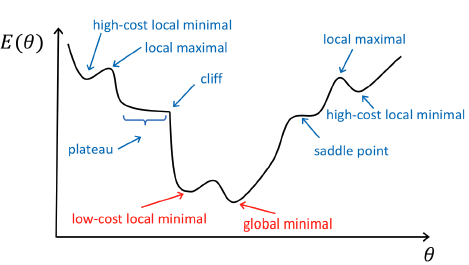
\includegraphics[width=0.8\linewidth]{fig/optim.png}
\end{figure}

\textbf{Responsive activation function:} saturation of sigmoid: $O=\sigma(I)=\cfrac{1}{1+exp(-I)}$; derivative: $\cfrac{\partial O}{\partial I}=O(1-O)$; error: $\delta_j=O_j(1-O_j)(O_j-T_j)$. If $O_j$ is close to 0 or 1, bother derivative and error is close 0 (gradient vanishing). 

ReLU: $O=I if I >0, otherwise 0$. No decaying in error, avoid gradient vanishing. 

\textbf{Adaptive learning rate}: SGD $\theta_{t+1}=\theta_t-\eta g_t$. Potential problems: slow progress, jump over gradient cliff; oscillation. Strategy: 1. $\eta_t=\cfrac{1}{t}\eta_0$; 2. $\eta_t=(1-t/T)\eta_0+t/T\eta_\infty$; 3. AdaGrad: $\eta_t=\cfrac{1}{\rho+r_i}\eta_0, r_i=\sqrt{\sum_{k=1}^t-1{g_{i,k}^2}}$. Intuition: the magnitude of gradient $g_t$ as the indicator of overall progress. 

\textbf{Dropout}: to prevent overfitting by randomly dropout of some non-output units. Regularization; Force the model to be more robust to noise, and to learn more generalizable features. 
VS bagging: each model is trained independently, while the model of current dropout network are updated based on previous dropout network.

\textbf{Pre-training}: the process of initializing the model in a suitable region. Greedy supervised pretraining; pre-set model parameters layer-by-layer in a greedy way; unsupervised pretraining: auto-encoder; hybrid. 

\textbf{Cross-entropy}: MSE for regression. CE Loss $-Tlog(O)-(1-T)log(1-O)$; error: $O-T$
% \begin{figure}[!ht]
%     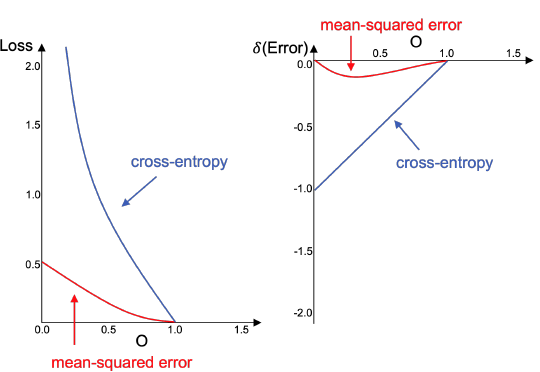
\includegraphics[width=0.8\linewidth]{fig/ce.png}
% \end{figure}

\section{CNN}
Challenges of MLP: Long training time, slow convergence, local minima. Motivation: Sparse interactions (Units in deeper layers still connect to a wide range of inputs); Parameter sharing (Reduce parameters); Translational equivalence $f(g(x))=g(f(x))$. CNN layer followed by non-linear activation and pooling. The deeper the better: learn from a larger receptive field.

\textbf{Pooling}: Introduces invariance to local translations; Reduces the number of hidden units in hidden layer

\section{RNN}
Handle sequence. $h^t=f(Ux^t, Wh^{t-1}+a)$; $\hat{y}^T=g(Vh^T+b)$. Recurrence to capture long-term dependence: same hidden-to-hidden matrix W; same input-to-hidden matrix U, same bias a. VS CNN: localized dependence. 

Challenges: long-term dependence. It needs deep RNN, leading to gradient vanishing or exploding. Solution: Gated RNN (LSTM, GRU) or attention mechanism. 

\textbf{LSTM}: cell state; accumulate the information from the past; three gate to control info flow (forget; input; output). 
\begin{figure}[!ht]
    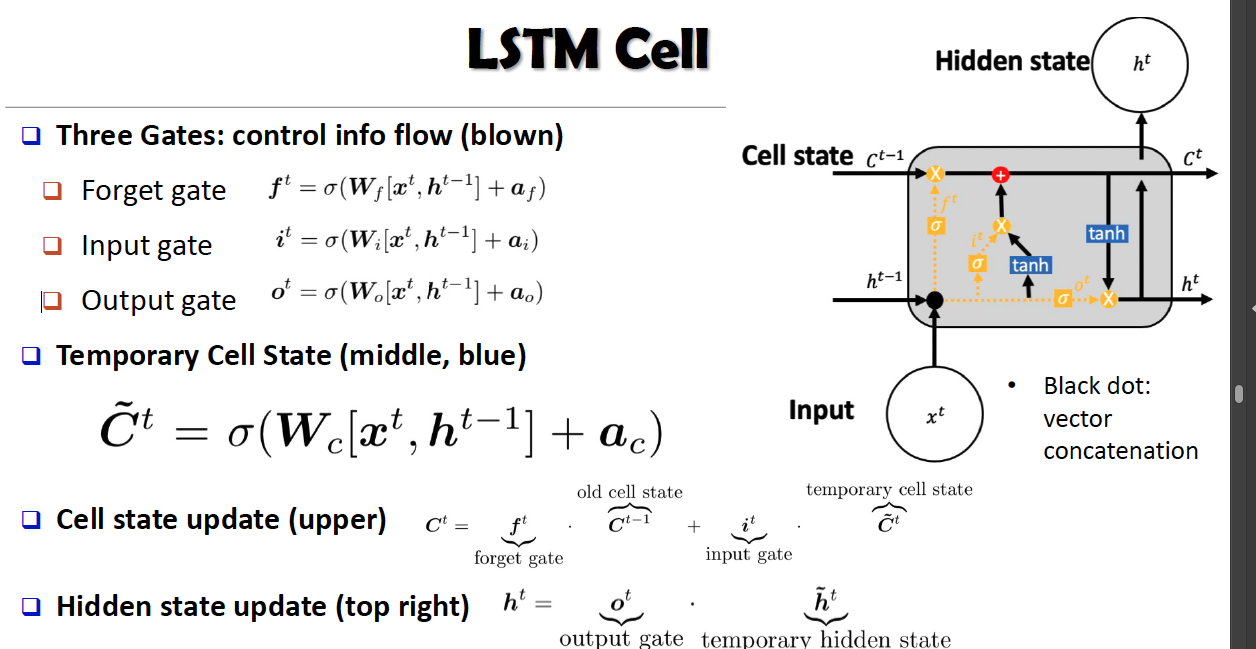
\includegraphics[width=\linewidth]{fig/lstm.png}
\end{figure}

\textbf{Attention}: Key Idea of Attention Mechanism: context vectors. Augment hidden state of 2nd RNN with context vectors. Introduce an alignment vector a and use linear weighted sum to obtain context vector. 

\section{GNN}
Challenges: Irregular graph structure (non-Euclidean): Unfixed size of node neighborhoods; Permutation invariance: Node ordering does not matter; Undefined convolution computation

\textbf{Graph convolution in spectral domain}: spectral-based model (GCN): $x*_\theta y\approx \theta(\tilde{D}^{-1/2}\tilde{A}\tilde{D}^{-1/2})x,\tilde{A}=A+I_n$

\begin{figure}[!ht]
    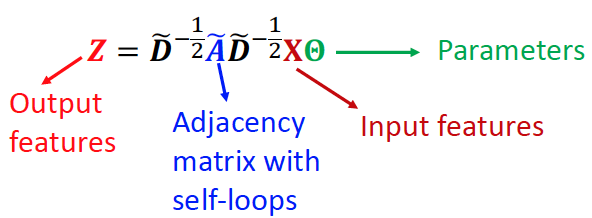
\includegraphics[width=\linewidth]{fig/gcn.png}
\end{figure}

A two-layer architecture for node classification: $\tilde{Y}=softmax(\hat{A}\sigma(\hat{A}X\theta_1)\theta_2),\hat{A}=\tilde{D}^{-1/2}\tilde{A}\tilde{D}^{-1/2}$

\textbf{Graph convolution in spatial domain}: $x(i)=w_{i,i}x(i)\sum_{j\in(i,k)}w_{i,j}x(j)$, where N is the k-hop neighborhood. key idea: message passing: how to aggregate node representations.


\section{Outlier}
Global Outliers (=point anomalies); Contextual Outliers (=conditional outliers); Collective Outliers (=group anomaly)
Challenge: Difficulty in modeling normality, ambiguity between normal and abnormal. Application-specific outlier detection; noise vs outlier (Noise: unavoidable, less interesting to the users, but make outlier detection more challenge); model interpretability. 

\textbf{Statistical approaches}: Assume
normal data are generated by a stochastic process Data objects in low density regions are flagged as outlier. 
Parametric Methods: The normal data objects are generated by a parametric distribution with a finite number of parameters: Single Variable Data: Grubb's test; Multi variable Data: Mahalanobis distance; $\chi^2$-statistics; mixture models
Non Parametric Methods: Do not assume a priori statistical model with a finite number of parameters: Outlier Detection by Histogram (Construct
histogram data objects outside bins are outliers); Outlier Detection by Kernel Density Estimation (Kernel
function: influence of a sample within its neighbor)

\textbf{Proximity-based approaches}: Intuition:
objects that are far from others can be regarded as outliers. Assumption: the proximity of an outlier object to its nearest neighbors significantly deviates from the proximity of most other objects to their nearest neighbors

\textbf{Distance-based outlier detection}: Consult the neighborhood of a sample. Outlier: if there are not enough objects in its neighborhood. 
r: distance threshold; $\pi$: fraction threshold. o is a $DB(r,\pi)$ -outlier if $\cfrac{\|\{o'|dist(o,o')\le r\}\|}{\|D\|}\le \pi$. Equivalent criteria: if $dist(o,o_k)>r$. $o_k$ is the k-nearest neighbor of o; $k=\lceil\pi\|D\|\rceil$


\end{document}